\documentclass[a4paper,12pt]{report}
\usepackage{mathtext}
\usepackage[T2A]{fontenc}
\usepackage[utf8]{inputenc}
\usepackage[english,russian]{babel}
\usepackage{geometry}
\usepackage{listings}
\usepackage{amsmath}
\geometry{top=2cm}
\usepackage{titlesec}
\usepackage{color}
\usepackage{pgfplots}
\usepackage{filecontents}
\usetikzlibrary{datavisualization}
\usetikzlibrary{datavisualization.formats.functions}
\usepackage{caption}
\DeclareCaptionFont{white}{\color{white}}
\DeclareCaptionFormat{listing}{\colorbox{gray}{\parbox{\textwidth}{#1#2#3}}}
\captionsetup[lstlisting]{format=listing,labelfont=white,textfont=white}

% Для листинга кода:
\lstset{ %
language=C++,                 % выбор языка для подсветки
basicstyle=\small\sffamily, % размер и начертание шрифта для подсветки кода
numbers=left,               % где поставить нумерацию строк (слева\справа)
numberstyle=\tiny,           % размер шрифта для номеров строк
stepnumber=1,                   % размер шага между двумя номерами строк
numbersep=-5pt,                % как далеко отстоят номера строк от подсвечиваемого кода
showspaces=false,
backgroundcolor=\color{white},         
showstringspaces=false,      % показывать или нет пробелы в строках
showtabs=false,             % показывать или нет табуляцию в строках
frame=single,              % рисовать рамку вокруг кода
tabsize=2,                 % размер табуляции по умолчанию равен 2 пробелам
captionpos=t,              % позиция заголовка вверху [t] или внизу [b] 
breaklines=true,           % автоматически переносить строки (да\нет)
breakatwhitespace=false, % переносить строки только если есть пробел
escapeinside={\%*}{*)},   % если нужно добавить комментарии в коде
	    keywordstyle=\color{blue}\ttfamily,
	    stringstyle=\color{red}\ttfamily,
	    commentstyle=\color{orange}\ttfamily,
	    morecomment=[l][\color{magenta}]{\#},
	    columns=fullflexible   % если нужно добавить комментарии в коде
}

% Для измененных титулов глав:
\definecolor{gray75}{gray}{0.75} % определяем цвет
\newcommand{\hsp}{\hspace{20pt}} % длина линии в 20pt
% titleformat определяет стиль
\titleformat{\chapter}[hang]{\Huge\bfseries}{\thechapter\hsp\textcolor{gray75}{|}\hsp}{0pt}{\Huge\bfseries}


\begin{document}
\begin{titlepage}
	\centering
	{\scshape\LARGE МГТУ им. Н.Э.Баумана \par}
	\vspace{4cm}
	{\scshape\Large Лабораторная работа №6\par}
	\vspace{0.5cm}	
	{\scshape\Large По курсу: "Анализ алгоритмов"\par}
	\vspace{2cm}
	{\huge\bfseries Муравьиный алгоритм\par}
	\vspace{3cm}
	\Large Работу выполнил: Луговой Дмитрий, ИУ7-51Б\par
	\vspace{0.5cm}
	\Large Преподаватель:  Волкова Л.Л.\par

	\vfill
	\large \textit {Москва, 2019} \par
\end{titlepage}

\setcounter{page}{2}

\tableofcontents

\newpage
\chapter*{Введение}
\addcontentsline{toc}{chapter}{Введение}
\hspace{0.6cm}  \textbf{Задача коммивояжера} формулируется как задача поиска минимального по стоимости замкнутого маршрута по всем вершинам без повторений на полном взвешенном графе с n вершинами. Содержательно вершины графа являются городами, которые должен посетить коммивояжер, а веса ребер отражают расстояния (длины) или стоимости проезда. \\

\textbf{Цель работы}: изучить муравьиный алгоритм по материалам решения задачи коммивояжера.\\\\

\textbf{\LARGE Задачи работы}\\\\
Задачами данной лабораторной являются:
\begin{enumerate}
\item[1)] Описать методы решения.
\item[2)] Реализовать алгоритм и описать полученные результаты.
\item[3)] Выбрать класс данных и составить набор данных.
\item[4)] Провести параметризацию метода на основе муравьиного алгоритма для выбранного класса данных.
\item[5)] Провести сравнительный анализ двух методов.
\item[6)] Дать рекомендации о применимости метода решения задачи коммивояжера на основе муравьиного алгоритма.
\end{enumerate}


\chapter{Аналитическая часть}
\hspace{0.6cm}В данном разделе содержится описание задачи коммивояжера и  методы её решения.
\section{Задача коммивояжера}
\hspace{0.6cm}В общем случае задача коммивояжера (странствующего торговца) может быть сформулирована следующим образом: найти самый выгодный (самый короткий, самый дешевый, и т.п.) маршрут, начинающийся в исходном городе и проходящий ровно один раз через каждый из указанных городов, с последующим возвратом в исходный город.

Проблему коммивояжера можно представить в виде модели на графе, то есть, используя вершины и ребра между ними. Таким образом, M вершин графа соответствуют M городам, а ребра $(i, j)$ между вершинами $i$ и $j$ — пути сообщения между этими городами. Каждому ребру $(i, j)$ можно сопоставить критерий выгодности маршрута $c_{ij} \geq 0$,который можно понимать как, например, расстояние между городами, время или стоимость поездки.  В целях упрощения задачи и гарантии существования маршрута обычно считается, что модельный граф задачи является полностью связным, то есть, что между произвольной парой вершин существует ребро.

Гамильтоновым циклом называется маршрут, включающий ровно по одному разу каждую вершину графа. Таким образом, решение задачи коммивояжёра — это нахождение гамильтонова цикла минимального веса в полном взвешенном графе.

\section{Стандартный алгоритм}

\hspace{0.6cm}Пусть  дано M - число городов, D - матрица смежности, каждый элемент которой - вес пути из одного города в другой. Существует метод грубой силы решения поставленной задачи, а именно полный перебор всех возможных гамильтоновых циклов в заданном графе с нахождением минимального по весу. Этот метод гарантированно даст идеальное решение (глобальный минимум по весу). Однако стоит учитывать, что сложность такого алгоритма составляет M! и время выполнения программы, реализующий такой подход, будет расти экспоненциально в зависимости от размеров входной матрицы.

\section{Муравьиный алгоритм}

\hspace{0.6cm}
Поскольку на практике чаще всего необходимо получить решение как можно быстрее, при этом требуемое решение не обязательно должно быть наилучшем, был разработан ряд методов, называемых эвристическими, которые решают поставленную задачу за гораздо меньшее время, чем метод полного перебора. В основе таких методов лежат принципы из окружающего мира, которые в дальнейшем могут быть формализованы.

Одним из таких методов является муравьиный метод. Он применим к решению задачи коммивояжера и основан на идее муравейника. Модель данного метода: у муравья есть 3 чувства:
\begin{itemize}
\item зрение (муравей может оценить длину ребра);
\item обоняние (муравей может унюхать феромон - вещество, выделяемое муравьем, для коммуникации с другими муравьями);
\item память (муравей запоминает свой маршрут).
\end{itemize}
Благодаря введению обоняния между муравьями возможен непрямой обмен информацией.

Введем вероятность $P_{k, ij}(t)$ выбора следующего города $j$ на маршруте муравьем $k$, который в текущий момент времени $t$ находится в городе $i$.
\begin{equation}\label{form:way} 
 p_{i,j}={\frac {(\tau _{i,j}^{\alpha })(\eta _{i,j}^{\beta })}{\sum (\tau _{i,j}^{\alpha })(\eta _{i,j}^{\beta })}}
 \end{equation}
 \begin{align*}
    \text{где} \\
   \tau _{i,j} &- \text{ феромон на ребре ij;} \\
    \eta _{i,j} &- \text{ привлекательность города j;} \\
    \alpha &- \text{параметр влияния длины пути;} \\
    \beta &- \text{параметр влияния феромона.}
\end{align*}

Очевидно, что при $\beta = 0$ алгоритм превращается в классический жадный алгоритм, а при $\alpha = 0$ он быстро сойдется к некоторому субоптимальному решению. Выбор правильного соотношения параметров является предметом исследований, и в общем случае производится на основании опыта.

После того, как муравей успешно проходит маршрут, он оставляет на всех пройденных ребрах феромон, обратно пропорциональный длине пройденного пути:
\begin{equation}\label{form:add} 
    \Delta \tau _{k, ij}= {\frac{Q}{L_{k}}}
\end{equation}
\begin{align*}
    \text{где} \\
    Q &- \text{количество феромона, переносимого муравьем;} \\
    L_{k} &- \text{стоимость k-го пути муравья (обычно длина).}
\end{align*}

После окончания условного дня наступает условная ночь, в течение которой феромон испаряется с ребер с коэффициентом $\rho$. Количество феромона на следующий день вычисляется по следующей формуле:
\begin{equation}\label{form:eva} 
    \tau _{i,j}(t+1)=(1-\rho )\tau _{i,j}(t)+\Delta \tau _{i,j}(t),
\end{equation}
\begin{align*}
    \text{где} \\
    \rho _{i,j} &- \text{доля феромона, который испарится;} \\
    \tau _{i,j}(t) &- \text{количество феромона на дуге ij;} \\
    \Delta \tau _{i,j}(t) &- \text{количество отложенного феромона.}
\end{align*}

Таким образом, псевдокод муравьиного алгоритма можно представить так:
\begin{enumerate}
\item Ввод матрицы расстояний D, количества городов M;
\item Инициализация параметров алгоритма — $\alpha$ $\beta$, $Q$, $tmax$, $\rho$;
\item Инициализация ребер — присвоение “привлекательности” $\eta_{ij}$ и начальной концентрации феромона  $\tau_{start}$;
\item	Размещение муравьев в случайно выбранные города без совпадений;
\item	Инициализация начального кратчайшего маршрута $L_{p}$ = null и определение длины кратчайшего маршрута $L_{min}$ = inf;
\item	Цикл по времени жизни колонии t = 1, tmax;
\begin{enumerate}
\item	Цикл по всем муравьям k = 1, M;
\begin{enumerate}
\item	Построить маршрут $T_{k}(t)$ по правилу 1.1  и рассчитать длину получившегося маршрута $L_{k}(t)$;
\item	Обновить феромон на маршруте по правилу 1.2;
\item	Если $L_{k}(t)$ < $L_{min}$, то $L_{min}$ = $L_{k}(t)$ и $L_{p} = T_{k}(t)$;
\end{enumerate}
\item	Конец цикла по муравьям;
\item Цикл по всем ребрам графа;
\begin{enumerate}
\item Обновить следы феромона на ребре по правилу 1.3;
\end{enumerate}
\item Конец цикла по ребрам;
\end{enumerate}
\item Конец цикла по времени;
\item Вывести кратчайший маршрут $L_{p}$ и его длину $L_{min}$.
\end{enumerate}

\section{Вывод}
\hspace{0.6cm}Таким образом, существуют две группы методов для решения задачи коммивояжера - точные и эвристические. К точным относится метод полного перебора, к эвристическим - муравьиный метод. Применение муравьиного алгоритма обосновано в тех случаях, когда необходимо быстро найти решение или когда для решения задачи достаточно получения первого приближения. В случае необходимости максимально точного решения используется алгоритм полного перебора.

\chapter{Конструкторская часть}
\hspace{0.6cm}В этом разделе содержатся схемы алгоритмов решения задачи коммивояжера.

\section{Схемы алгоритмов}

\hspace{0.6cm}На рисунках 2.1 и 2.2 представлена схема муравьиного алгоритма.

\begin{figure}[ht!]
\center{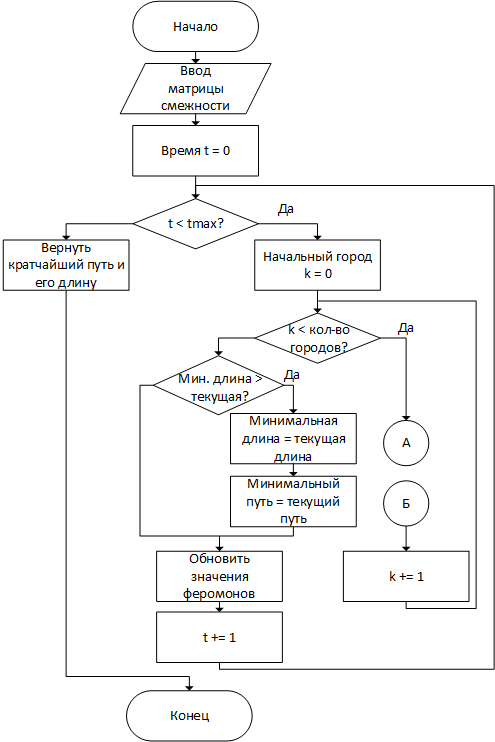
\includegraphics[scale=0.73]{Ant1.png}}
\caption{Схема муравьиного алгоритма}
\end{figure}
\newpage
\begin{figure}[ht!]
\center{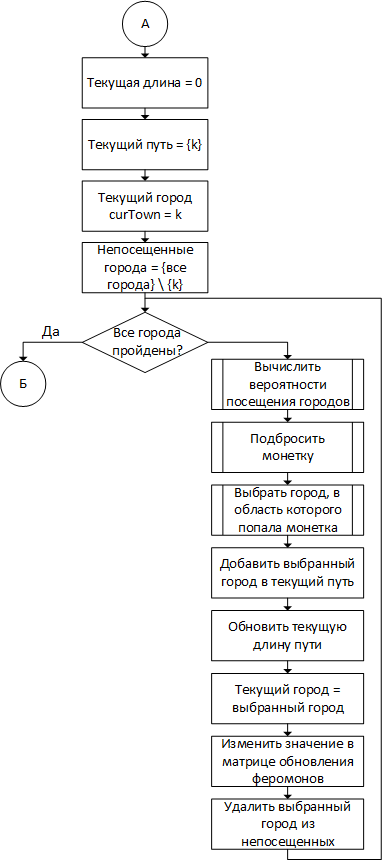
\includegraphics[scale=0.9]{Ant2.png}}
\caption{Схема муравьиного алгоритма(продолжение)}
\end{figure}

\newpage

На рисунке 2.3 представлена схема основной части алгоритма полного перебора.

\begin{figure}[ht!]
\center{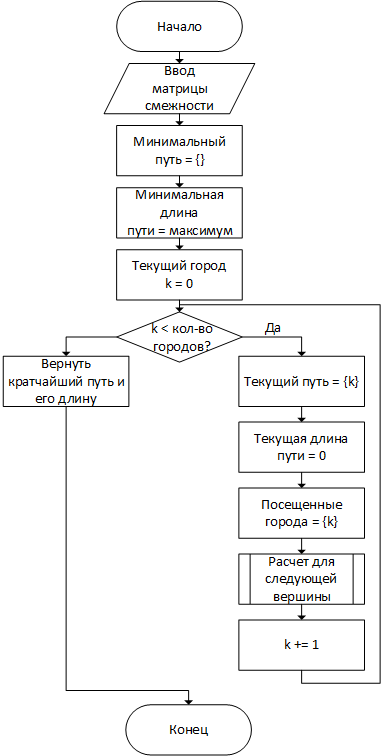
\includegraphics[scale=0.9]{Brute1.png}}
\caption{Схема основной части алгоритма полного перебора}
\end{figure}

\newpage

На рисунке 2.4 представлена схема рекурсивной части алгоритма полного перебора.

\begin{figure}[ht!]
\center{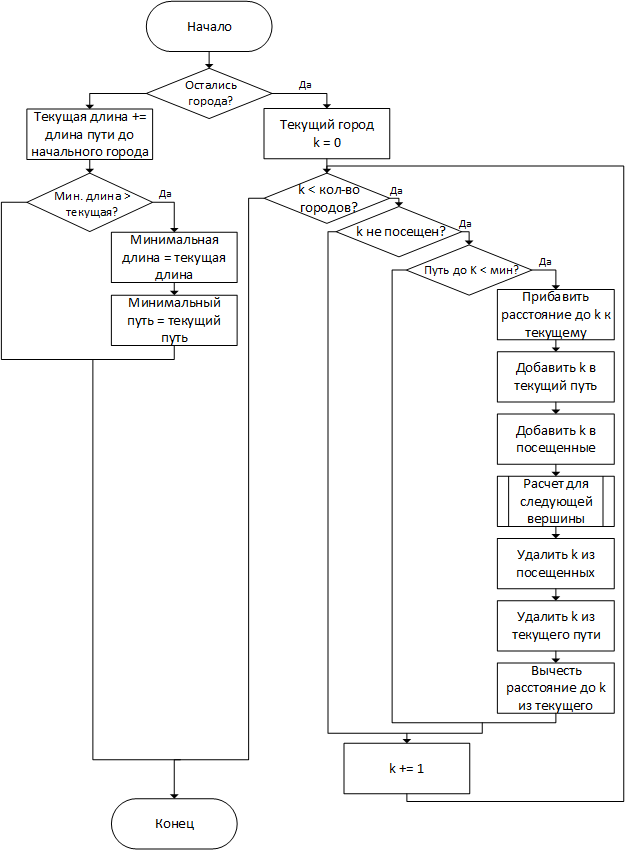
\includegraphics[scale=0.9]{Brute2.png}}
\caption{Схема рекурсивной части алгоритма полного перебора}
\end{figure}

\newpage

\section{Вывод}

\hspace{0.6cm}Как видно из схем алгоритмов, количество блоков операций над данным в алгоритме полного перебора меньше, чем в муравьином. Это объясняется более сложной моделью данных в случае муравьиного метода. При этом стоит отметить, что в стандартный алгоритм полного перебора внесено одно изменение, а именно проверка текущей длины пути: если она уже больше длины минимального на текущий момент маршрута, то дальше маршрут по этому пути не строится. Такая модификация позволяет увеличить быстродействие программы.

\chapter{Технологическая часть}
\hspace{0.6cm}В данном разделе приведены требования к программному обеспечению, средства реализации и листинги кода
\section{Требования к ПО}

\hspace{0.6cm}Программа на вход получает матрицу смежности графа. Выход  программы: последовательность целых чисел - минимальный по стоимости маршрут и действительное число - суммарная стоимость этого маршрута.
	
\section{Средства реализации}
\hspace{0.6cm}Для реализации представленных алгоритмов был выбран язык C++. Время работы алгоритмов было замерено с помощью функции system\_clock() из библиотеки chrono. Для тестирования использовался компьютер на базе процессора Intel Core i5 (4 физических ядра, 8 логических).

\section{Листинги кода}

\hspace{0.6cm}В процессе разработки программы был спроектирован шаблон класса Matrix,  служащий для работы с матрицей смежности, а также с матрицами для хранения количества феромона на ребрах.

В Листинге 3.1 показана реализация муравьиного алгоритма.

\begin{lstlisting}[caption=Функция муравьиного поиска кратчайшего пути]
    Route ant(const Matrix<double> &distances, const int &tMax, const double &alpha, const double &p)
    {
        const size_t nTowns = distances.size();
        // Pheromone coefficient
        const double q = distances.average() * nTowns;
        const double betta = 1 - alpha;
        // Attractions of the towns
        Matrix <double> attractions(distances);
        attractions.inverse();
        // Pheromones between towns
        Matrix<double> teta(nTowns, START_TETA);
        // Pheromone daily change
        Matrix<double> deltaTeta(nTowns);
    
        Route minRoute;
        minRoute.length = -1;
        std::vector<double> probabilities(nTowns, 0.0);
    
        for (int t = 0; t < tMax; t++)
        {
            // Day
            deltaTeta.zero();
            // Ants loop
            for (int k = 0; k < nTowns; k++)
            {
                std::vector<int> curPath = {k};
                double curLength = 0;
                int curTown = k;
    
                // Ants path
                std::vector<int> unvisited = getUnvisited(curPath, nTowns);
                while (curPath.size() != nTowns)
                {
                    fill(probabilities.begin(), probabilities.end(), 0.0);
    
                    // Probabilities of visiting towns
                    for (const auto &town : unvisited)
                    {
                        int index = getIndex(unvisited, town);
                        if (fabs(distances[curTown][town]) > EPS)
                        {
                            double sum = 0;
                            for (auto n : unvisited)
                                sum += pow(teta[curTown][n], alpha) * pow(attractions[curTown][n], betta);
                            probabilities[index] = pow(teta[curTown][town], alpha) * pow(attractions[curTown][town], betta) / sum;
                        }
                        else
                            probabilities[index] = 0;
                    }
    
                    // Choosing town
                    double coin = tossCoin();
                    size_t townIndex = 0;
                    double curProbability = 0;
                    for (size_t j = 0; j < nTowns; j++)
                    {
                        curProbability += probabilities[j];
                        if (coin < curProbability)
                        {
                            townIndex = j;
                            break;
                        }
                    }
                    int chosenTown = unvisited[townIndex];
                    curPath.push_back(chosenTown);
                    curLength += distances[curTown][chosenTown];
                    deltaTeta[curTown][chosenTown] += q / curLength;
                    curTown = chosenTown;
                    unvisited.erase(unvisited.begin() + townIndex);
                }
                // Update path
                curLength += distances[curPath[curPath.size() - 1]][curPath[0]];
                if (minRoute.length < -EPS || (curLength < minRoute.length))
                {
                    minRoute.length = curLength;
                    minRoute.path = curPath;
                }
            }
            // Night
            teta *= (1.0 - p);
            teta += deltaTeta;
            teta.replaceZero(MIN_TETA);
        }
        return minRoute;
    }
\end{lstlisting}

В Листингах 3.1 и 3.2 представлена реализация алгоритма полного перебора, представленная главной функцией bruteForce и рекурсивной hamilton.
\begin{lstlisting}[caption=Главная функция алгоритма полного перебора]
    Route bruteForce(const Matrix<double> &distances)
    {
        int n = distances.size();
        std::vector<bool> visited(n, false);
        std::vector<int> curPath;
        Route minRoute;
        minRoute.length = DBL_MAX;
        double curLen = 0;
        for (int i = 0; i < n; i++)
        {
            curPath.clear();
            curPath.push_back(i);
            fill(visited.begin(), visited.end(), 0);
            visited[i] = true;
            curLen = 0;
            hamilton(distances, minRoute, curPath, visited, curLen);
        }
        return minRoute;
    }
\end{lstlisting}

 Основная функция вызывает в цикле для каждой вершины рекурсивную функцию, в которой проверяются все непосещенные вершины и если такие есть, то эта  функция вызывается для следующих вершин пока не будет пройден полноценный маршрут.

\begin{lstlisting}[caption=Рекурсивная функция алгоритма полного перебора]
    void hamilton(const Matrix<double> &distances,Route &minRote, std::vector<int> &curPath, std::vector<bool> &visited, double &curLen)
    {
        if (curPath.size() == distances.size())
        {
            double tmp = distances[curPath.back()][curPath[0]];
            if (curLen + tmp < minRote.length)
            {
                minRote.path = curPath;
                minRote.length = curLen + tmp;
            }
            return;
        }
        for (int i = 0; i < distances.size(); i++)
        {
            if (!visited[i])
            {
                double tmp = distances[curPath.back()][i];
                if (curLen + tmp > minRote.length)
                    continue;
                curLen += tmp;
                curPath.push_back(i);
                visited[i] = true;
                hamilton(distances, minRote, curPath, visited, curLen);
                visited[i] = false;
                curPath.pop_back();
                curLen -= tmp;
            }
        }
    }
\end{lstlisting}

\section{Вывод}
\hspace{0.6cm}Были реализованы муравьиный алгоритм и алгоритм полного перебора, решающие задачу коммивояжера, для дальнейшего сравнительного анализа точности и скорости вычислений. 

\chapter{Экспериментальная часть}
\hspace{0.6cm}В данном разделе приведены примеры работы программы, проведена параметризация метода решения задачи коммивояжера на основе муравьиного алгоритма, а также проведен сравнительный анализ двух алгоритмов.
\section{Примеры работы}
\hspace{0.6cm}На рисунках 4.1 - 4.3 приведены примеры работы программы. В консоль выводится входная матрица смежности, длина кратчайшего маршрута и сам маршрут для двух алгоритмов.

\begin{figure}[ht!]
\center{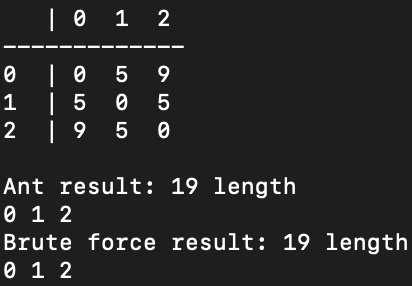
\includegraphics[scale=0.9]{Example3.png}}
\caption{Пример работы для матрицы 3x3}
\end{figure}

\begin{figure}[ht!]
\center{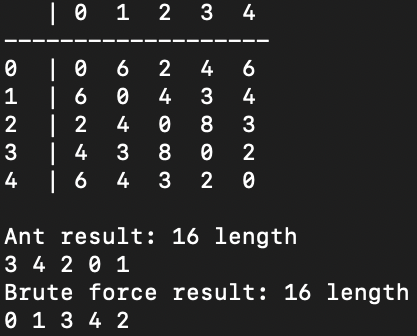
\includegraphics[scale=0.9]{Example5.png}}
\caption{Пример работы для матрицы 5x5}
\end{figure}

\begin{figure}[ht!]
\center{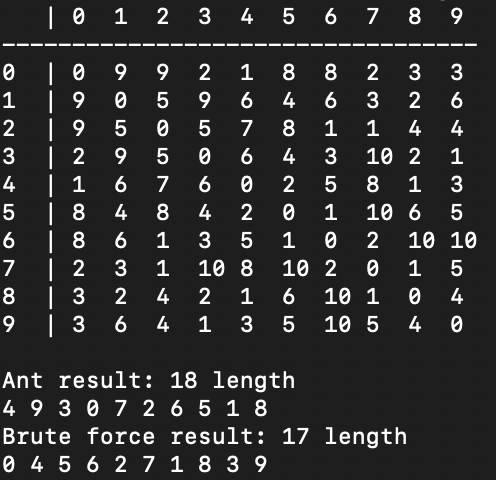
\includegraphics[scale=0.9]{Example10.png}}
\caption{Пример работы для матрицы 10x10}
\end{figure}

Как видно из приведенных примеров, с увеличением размерности матрицы, муравьиный алгоритм начинает показывать меньшую точность, в то время как полный перебор находит наилучший вариант в любом случае. 

\section{Анализ лога}

\hspace{0.6cm}

\section{Вывод}
\hspace{0.6cm} 

\newpage
\chapter*{Заключение}
\addcontentsline{toc}{chapter}{Заключение}
\hspace{0.6cm}
  
\end{document}